%%%%%%%%%%%%%%%%%%%%%%%%%%%%%%%%%%%%%%%%%
% Medium Length Professional CV
% LaTeX Template
% Version 2.0 (8/5/13)
%
% This template has been downloaded from:
% http://www.LaTeXTemplates.com
%
% Original author:
% Trey Hunner (http://www.treyhunner.com/)
%
% Important note:
% This template requires the resume.cls file to be in the same directory as the
% .tex file. The resume.cls file provides the resume style used for structuring the
% document.
%
%%%%%%%%%%%%%%%%%%%%%%%%%%%%%%%%%%%%%%%%%

%----------------------------------------------------------------------------------------
%	PACKAGES AND OTHER DOCUMENT CONFIGURATIONS
%----------------------------------------------------------------------------------------

\documentclass{resume} % Use the custom resume.cls style

\usepackage[left=0.65in,top=0.5in,right=0.65in,bottom=0.5in]{geometry} % Document margins
\usepackage{hyperref}
\usepackage{array} 
\usepackage{textpos}
\usepackage[utf8]{inputenc}
\usepackage{graphicx}
\usepackage[russian,english]{babel}

\begin{textblock}{7}(0, 0.05)
{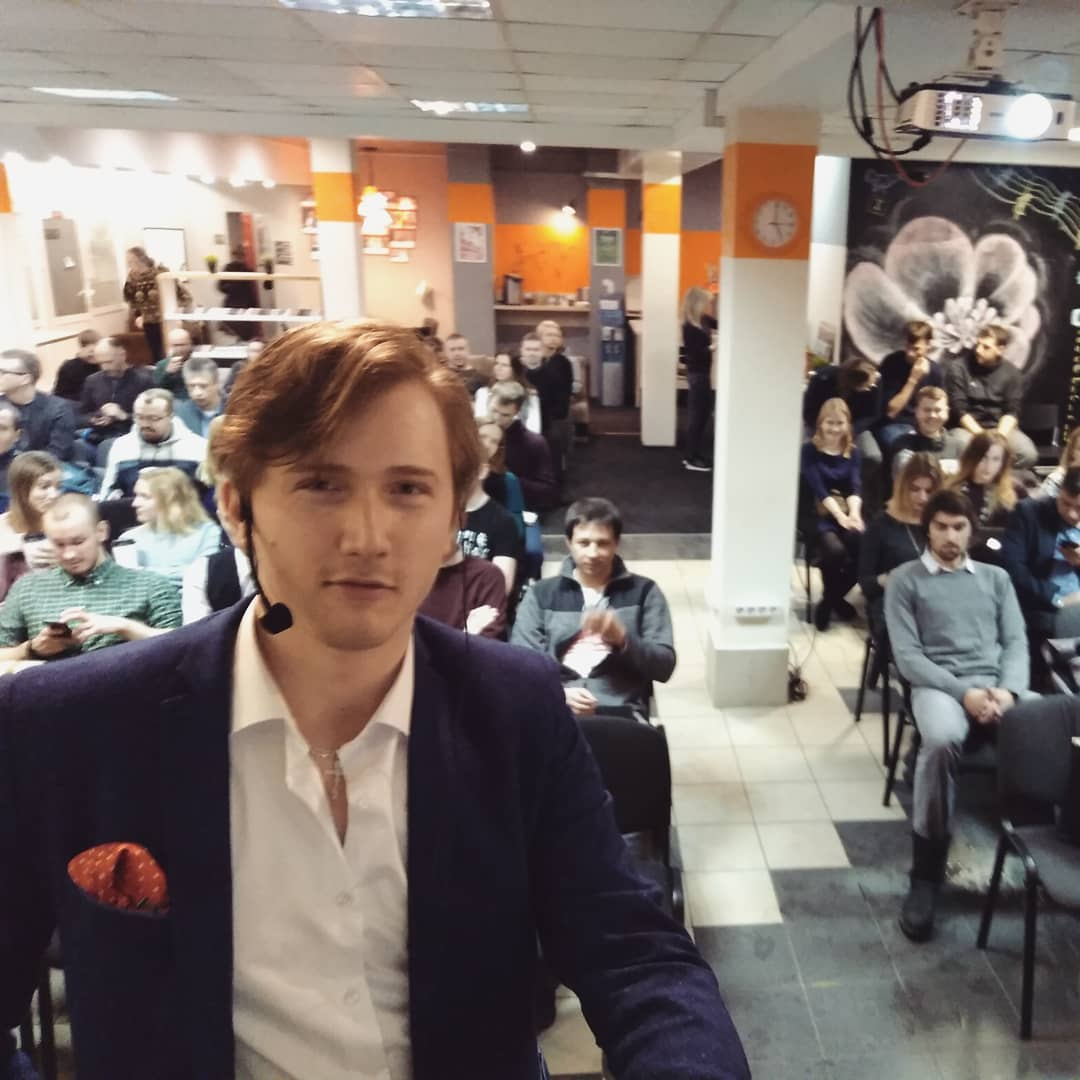
\includegraphics[width=.23\linewidth]{photo.jpg}}
\end{textblock}

\name{Alexander Mikhalchenko} % Your name
\address{Belarus, Minsk 220113} % Your address
\address{Linkedin: \href{http://linkedin.com/in/mikhalchenkoa}{linkedin.com/in/mikhalchenkoa}  SO: \href{http://stackoverflow.com/users/2044039}{stackoverflow.com/users/2044039}} \\
\address{alexander.a.mikhalchenko@gmail.com \\ skype:strrife } % Your phone number and email

\begin{document}

%----------------------------------------------------------------------------------------
%	SUMMARY SECTION
%----------------------------------------------------------------------------------------

\begin{rSection}{Summary}

I'm skilled fast-learning developer with a strong mathematical background constantly looking for ways to apply and enrich my knowledge. Over the past years I have worked with a variety of web technologies and I'm experenced in backend, frontend, databases and software architecture. I have good communication skills and ~2 years of working in different teams.

\end{rSection}


%----------------------------------------------------------------------------------------
%	TECHNICAL STRENGTHS SECTION
%----------------------------------------------------------------------------------------

\begin{rSection}{Technical Strengths}

\begin{tabular}{ @{} >{\bfseries}l @{\hspace{4ex}} l }
JavaScript (3 years) & ES6, Angular, Aurelia, JSPM, Bower, jQuery, Isomorphic apps, React \\
NodeJS (1 year) & Express, NPM, Grunt, Gulp, Yeoman, Browserify, JSLint \\
PHP 5.3+ (3 years), PHP7 & Symfony 2, Symfony 1.4, Wordpress, Silex, Composer, Doctrine, PDO \\
MySQL, SQLite (2 years) & MySQLi, InnoDB; Raw and with ORMs \\
MongoDB, Redis (1 year) & ElasticSearch, Mongoose, MapReduce \\
HTML/XML (3 years) & HTML5, DOM, Schema, SAX, Canvas \\
CSS (2 years) & SASS, LESS, CSS3, Bootstrap, Flat UI \\
Testing & Mocha, Karma, Selenium, PHPUnit, Nightmare.js \\
Other & AWS (EC, S3, SQS), Python (NumPy, OpenCV), C/C++, C\# (.NET) \\
 & Java (Spring, Swing), lots of APIs (Dropbox, Google, Mangopay, etc) \\
VCS & Git, Perforce \\
\end{tabular}

\end{rSection}

%----------------------------------------------------------------------------------------
%	WORK EXPERIENCE SECTION
%----------------------------------------------------------------------------------------

\begin{rSection}{Work experience}

\begin{rSubsection}{DualLab}{August 2015 - Present}{Full stack Web Developer}{Minsk, Belarus}
\item Was responsible for development of the web client and the REST API on top of the legacy SOAP API
\item NodeJS + Express used for backend, Angular for frontend 
\item Test-driven development (Nightmare.js and Mocha for testing)
\item Agile Software Development (Scrum)
\item Recommendations from my team leader and colleagues can be found on my \href{http://linkedin.com/in/mikhalchenkoa}{linkedin profile}
\end{rSubsection}

%------------------------------------------------

\begin{rSubsection}{StarOfService}{April 2014 - August 2015}{Full stack Web Developer}{Paris, France}
\item PHP, Symfony 1.4 for backend; Angular, jQuery for frontend
\item integration with AWS (SQS in particular)
\item Data mining: TF-IDF-based search engine for the homepage, Mixpanel, duplicate requests detector
\item REST API (designed by me from scratch) for the iPhone app 
\item Agile Software Development (Kanban)
\item Recommendations from the CEO, CTO and my team leader can be found on my \href{http://linkedin.com/in/mikhalchenkoa}{linkedin profile}
\end{rSubsection}
%------------------------------------------------

\begin{rSubsection}{Athena Art}{February 2014 - April 2014}{Wordpress Developer}{Italy, Torino}
\item Wordpress customization (creating custom post type managers)
\item Load speed optimization (page load time reduced from 1.5s to 0.03s with custom redis-based solution)
\end{rSubsection}
%------------------------------------------------

\begin{rSubsection}{Itransition}{October 2013 - January 2014}{PHP developer}{Minsk, Belarus}
\item Symfony web developer (traineeship + work)
\item Symfony 2.2 as backend, jQuery + Bootstrap 3 as frontend, worked on a shop catalog system
\end{rSubsection}

\end{rSection}

\clearpage

%----------------------------------------------------------------------------------------
%	Other projects
%----------------------------------------------------------------------------------------

\begin{rSection}{Other projects I worked on}

{\bf \href{http://toto.by}{ToTo.by}} \hfill {\em since November 2015} \\ 
My friend's project that organizes and accumulates all car-related information in Belarus, helping people with the rutine of finding service stations, selling and buying vehicles.\\

{\bf \href{http://pirateminds.com/e-analytics}{E-Analytics}} \hfill {\em October 2015} \\ 
BI application with recommendation engine for retail and e-commerce (business analysis, feasibility study, marketing research) \\

{\bf \href{http://boxinator.xyz}{Boxinator}} \hfill {\em September 2015} \\ 
Cloud-based workflow management system developed with NodeJS using Dropbox API. Presented at Minsk FinTech hackaton. \\

{\bf \href{http://mmopricefinder.com}{MMOPriceFinder.com}} \hfill {\em July 2014} \\ 
Dynamically updating World of Warcraft and other games inner currency rates. Developed with Symfony 2, Angular JS and Flat UI \\

\end{rSection}

%----------------------------------------------------------------------------------------

%----------------------------------------------------------------------------------------
%	EDUCATION SECTION
%----------------------------------------------------------------------------------------

\begin{rSection}{Education}

{\bf Belarussian State University, Belarus} \hfill {\em 2012 $-$ Present} \\ 
Bachelor Degree in Computer Science \& Mathematics \\
Minor in Intelligent Control Systems \smallskip \\
Courses taken: Algorithms, Pattern recognition, Natural Text Processing, Calculus, etc. \smallskip \\
Average: 9.47

{\bf Belarussian State University Lyceum, Belarus} \hfill {\em 2010 $-$ 2012} \\ 
Associate degree in Mathematics \\
Average: 9.8

\end{rSection}

%----------------------------------------------------------------------------------------
%	Mathematics
%----------------------------------------------------------------------------------------

\begin{rSection}{Mathematical activities}

\begin{rSubsection}{International Tournaments of Young Mathematicians}{}{}

\item ITYM 4 $-$ 1st place \& gold medal \hfill July 2012, Paris, France
\item ITYM 6 $-$ 2nd place \& gold medal (team leader) \hfill July 2014, Bremen, Germany

\end{rSubsection}

\begin{rSubsection}{Belarussian Mathematical Olympiads}{}{}

\item 61st BMO $-$ I diploma \hfill  April 2011, Belarus, Gomel
\item 62nd BMO $-$ II diploma \hfill April 2012, Belarus, Gomel
\end{rSubsection}


\begin{rSubsection}{Local Tournaments of Young Mathematicians}{}{}

\item XIV Belarussian TYM $-$ 1st place (team leader) \hfill December 2012, Belarus, Minsk
\item XV Belarussian TYM $-$ 1st place (team leader) \hfill December 2013, Belarus, Minsk
\item 2nd St.Petersburg TYM $-$ 1st place (team leader) \hfill March 2014, Russia, St. Petersburg
\end{rSubsection}

\end{rSection}

\begin{rSection}{Publications}

{\bf "Sentimental corpus of texts generating system for solving semantic web problems in tourism domain"}
% ("Система синтеза сентиментального корпуса текста для решения задач semantic web в области туризма")%. 

Presented at the 72th BSU Scientific Conference (May 15, 2015). Approved for publication, is to be published before the 73rd BSU Scientific Conference.

\end{rSection}


%----------------------------------------------------------------------------------------
%	EXAMPLE SECTION
%----------------------------------------------------------------------------------------

%\begin{rSection}{Section Name}

%Section content\ldots

%\end{rSection}

%----------------------------------------------------------------------------------------

\end{document}
